\documentclass[]{AVSSimReportMemo}
\usepackage{AVS}

\newcommand{\ModuleName}{orbitAxisSpin}
\newcommand{\subject}{Guidance Module to Perform a Constant Spinning about an Orbit Axis}
\newcommand{\status}{Initial Version}
\newcommand{\preparer}{M. Cols}
\newcommand{\summary}{Generate the attitude reference to achieve a spinning motion about a primary orbit frame axis. A chosen reference axis $\hat{r}_{j} = \hat{r}_{spin}$ is to line up with the orbit axis $\hat{o}_{i} = \hat{o}_{spin}$, and rotate a desired rate $\omega_{spin}$}


\begin{document}

\makeCover


%
%	enter the revision documentation here
%	to add more lines, copy the table entry and the \hline, and paste after the current entry.
%
\pagestyle{empty}
{\renewcommand{\arraystretch}{2}
\noindent
\begin{longtable}{|p{0.5in}|p{4.5in}|p{1.14in}|}
\hline
{\bfseries Rev}: & {\bfseries Change Description} & {\bfseries By} \\
\hline
Draft & initial copy & M. Cols \\
\hline

\end{longtable}
}

\newpage
\setcounter{page}{1}
\pagestyle{fancy}

\tableofcontents
~\\ \hrule ~\\

\begin{figure}[htb]
	\centerline{
	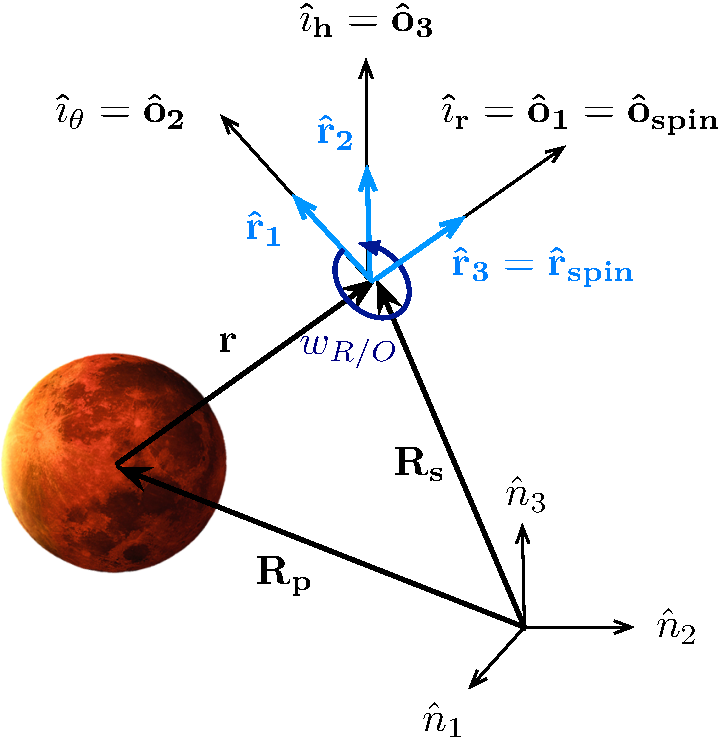
\includegraphics[width=5cm]{Figures/orbitSpin}
	}
	\caption{Illustration of having $\hat{r}_{3}$ aligned with $\hat{o}_{1}$ and spinning about it at a constant rate $\omega_{spin}$.}
	\label{fig:Fig1}
\end{figure}

\section{Introduction}
In this note a method is discussed on how to compute the reference frame angular rate $\bm\omega_{R/N}$ and acceleration $\dot{\bm\omega}_{R/N}$ to achieve a particular family of stabilized spin motion. A reference is already aligned with a principal orbit axis and the purpose of this module is to have the refernce spinning at a desired rate about the axis at which is pointing. Note that the presented method is general enough to use any of the Hill or Velocity orbit frames.\par
Figure 1 illustrates the following example. Here the reference axis $\hat{r}_{3}$ is to spin about $\hat{o}_{spin} = \hat{o}_{spin}$, which has been chosen to be the nadir axis $\hat{\imath}_{r}$ of the Hill reference frame.

\section{Angular Velocity and Acceleration Descriptions}
The reference frame $\mathcal{R}$ is defined above, and the attitude reference frame tracking control requires the angular rate $\bm\omega_{R/N}$ and acceleration $\dot{\bm\omega}_{R/N}$. 
Let the MRP attitude set, angular velocity vector and angular acceleration vector associated with a constant pointing be $\bm\sigma_{O/N}$, $\bm\omega_{O/N}$ and $\bm\dot{\omega}_{O/N}$ respectively.
As proved in Orbit Axis Pointing documentation,
\begin{equation}
	\label{eq:dbeta}
	\bm\omega_{O/N} = \dot f \hat{\bm\imath}_{h} 
\end{equation}
\begin{equation}
	\label{eq:dbeta}
	\bm{\dot\omega}_{O/N} = \ddot{f} \hat{\bm\imath}_{h}
\end{equation}
The angular velocity of the spinning reference frame is thus given by:
\begin{equation}
	\label{eq:dbeta}
	\bm\omega_{R/N} = \bm\omega_{spin} + \bm\omega_{O/N} = \omega_{spin}\bm\hat{o}_{spin} + \dot f \hat{\bm\imath}_{h} 
\end{equation}
Using the transport theorem, the angular acceleration vector is found to be
\begin{equation}
	\label{eq:dbeta}
	\bm{\dot\omega}_{R/N} = \frac{^\mathcal{O} d}{dt} (\omega_{spin}\bm\hat{o}_{spin}) + \bm\omega_{O/N}\times (\omega_{spin}\bm\hat{o}_{spin}) + \bm{\dot\omega}_{O/N}
\end{equation}
\begin{equation}
	\label{eq:dbeta}
	\bm{\dot\omega}_{R/N} = \bm\dot\omega_{spin}\bm\hat{o}_{spin} +  \dot{f}\omega_{spin}(\bm\hat{\imath}_{h} \times \bm\hat{o}_{spin})+ \ddot f \hat{\bm\imath}_{h} 
\end{equation}

\section{MRP Attitude Set}
Let be $\phi_{spin}$ be the current spin angle that the reference frame has rotated about its spin axis $\hat r_{spin}$. The final reference frame orientation is eventually given by
\begin{equation}
	\label{eq:dbeta}
	[RN] =  [M_{r_{spin}} (\phi_{spin})][ON]
\end{equation}
where [ON] is the Direction Cosine Matrix associated with the orbit axis pointing attitude set, and $M_{r_{spin}}$ is the principal axis rotation matrix about $\hat r_{spin}$. Assuming a constant spin rate, the spin angle is propagated using the simple Euler integration scheme
\begin{equation}
	\label{eq:dbeta}
	\phi_{spin, n+1} = \phi_{spin, n} + \omega_{spin}\Delta t
\end{equation}
With [RN] defined, the MRP attitude set $\sigma_{R/N}$ can readily be computed.

\section{Spin Angle Initialization Process}
The question remains on how to initialize the spin angle $\phi_{spin}$. At this point, the generalization of the method must be sacrificed, since the actual body axis that is about to spin is needed. Given the relative orientation between two frames, the current $\mathcal{B}$ and the desired $\mathcal{R}$, the principal rotation to achieve the aligmnent could be done along the principal rotation angle $\phi$ or $2\pi - \phi$. The aim of this process is to ensure that the path followed to achieve the frame alignment is the shortest.
\subsection{Algorithm Outline}
A separate algorithm is used to compute the initial spin angle. In this independent method, the frames are as follows:\par
Being $\hat{b}_{spin}$ the principal body axis that is to be aligned with the principal orbit frame axis $\hat{o}_{spin}$, the orbit frame is defined such that $\hat{o}_{1} = \hat{o}_{spin}$, while $\hat{o}_{2}$ and $\hat{o}_{3}$ are defined following either the LVLH or velocity orbit, i.e. $\mathcal{H}$ and $\mathcal{V}$ definitions. Note that the enumeration of the axes order rolls over to keep a right-handed coordinate frame. Similary, the principal reference axes indices are labeled using $\hat b_{i}$, where the first index $\hat b_{1}$ determines which reference axis is the final spin axis, i.e. $\hat b_{1} =\hat b_{spin}$. The remaining two indices are set to yield a right-handed coordinate frame.\par
To define the orbit frame orientation to line up the $\hat o_{1}$ orbit axis and $\hat b_{1}$ body axis, let us use the definition where ON($i$) is the $i_{th}$ row of the [ON] DCM matrix. We then set
\begin{equation}
	\label{eq:dbeta}
	ON(\hat b_{1}) = ON(\hat o_{1}) = \bm\hat\imath_{o_{1}}
\end{equation}
\begin{equation}
	\label{eq:dbeta}
	ON(\hat b_{2}) = ON(\hat o_{2}) = \bm\hat\imath_{o_{2}}
\end{equation}
\begin{equation}
	\label{eq:dbeta}
	ON(\hat b_{3}) = \bm\hat\imath_{o_{1}} \times \bm\hat\imath_{o_{2}}
\end{equation}
Having [ON] defined for a specific body frame and [BN], the computations are straightforward. First, the spin axis alignment angle is computed as the relative orientation between $\hat b_{spin}$ and $\hat o_{spin}$. Next, the body frame is rotated about a principal rotation angle to align these two axes. Eventually, the initial spin angle is defined as the angle to align the remaining 2 axes. This process results in the desired spin axis being the closes to the current body frame arrangement.

\bibliographystyle{unsrt}
\bibliography{references}

\end{document}
